\documentclass[10pt,a4paper]{scrartcl}
\usepackage[utf8]{inputenc}
\usepackage{amsmath}
\usepackage{amsfonts}
\usepackage{amssymb}
\usepackage{graphicx}

\usepackage[bottom = 1in, left = 0.5in, right = 0.5in, top = 1in]{geometry}

\usepackage[english]{babel}
\usepackage[autostyle]{csquotes}
\usepackage{mathptmx}

\usepackage[labelfont=bf]{caption}

\usepackage[default, scale=0.95]{opensans} %% Alternatively
%% use the option 'defaultsans' instead of 'default' to replace the
%% sans serif font only.
\usepackage[T1]{fontenc}

\addto\captionsenglish{\renewcommand{\figurename}{Supplementary Fig.}}

\title{My neat title here}
\subtitle{Supplementary materials}
\date{}

\begin{document}
\maketitle

\begin{figure}[h]
	\centering
	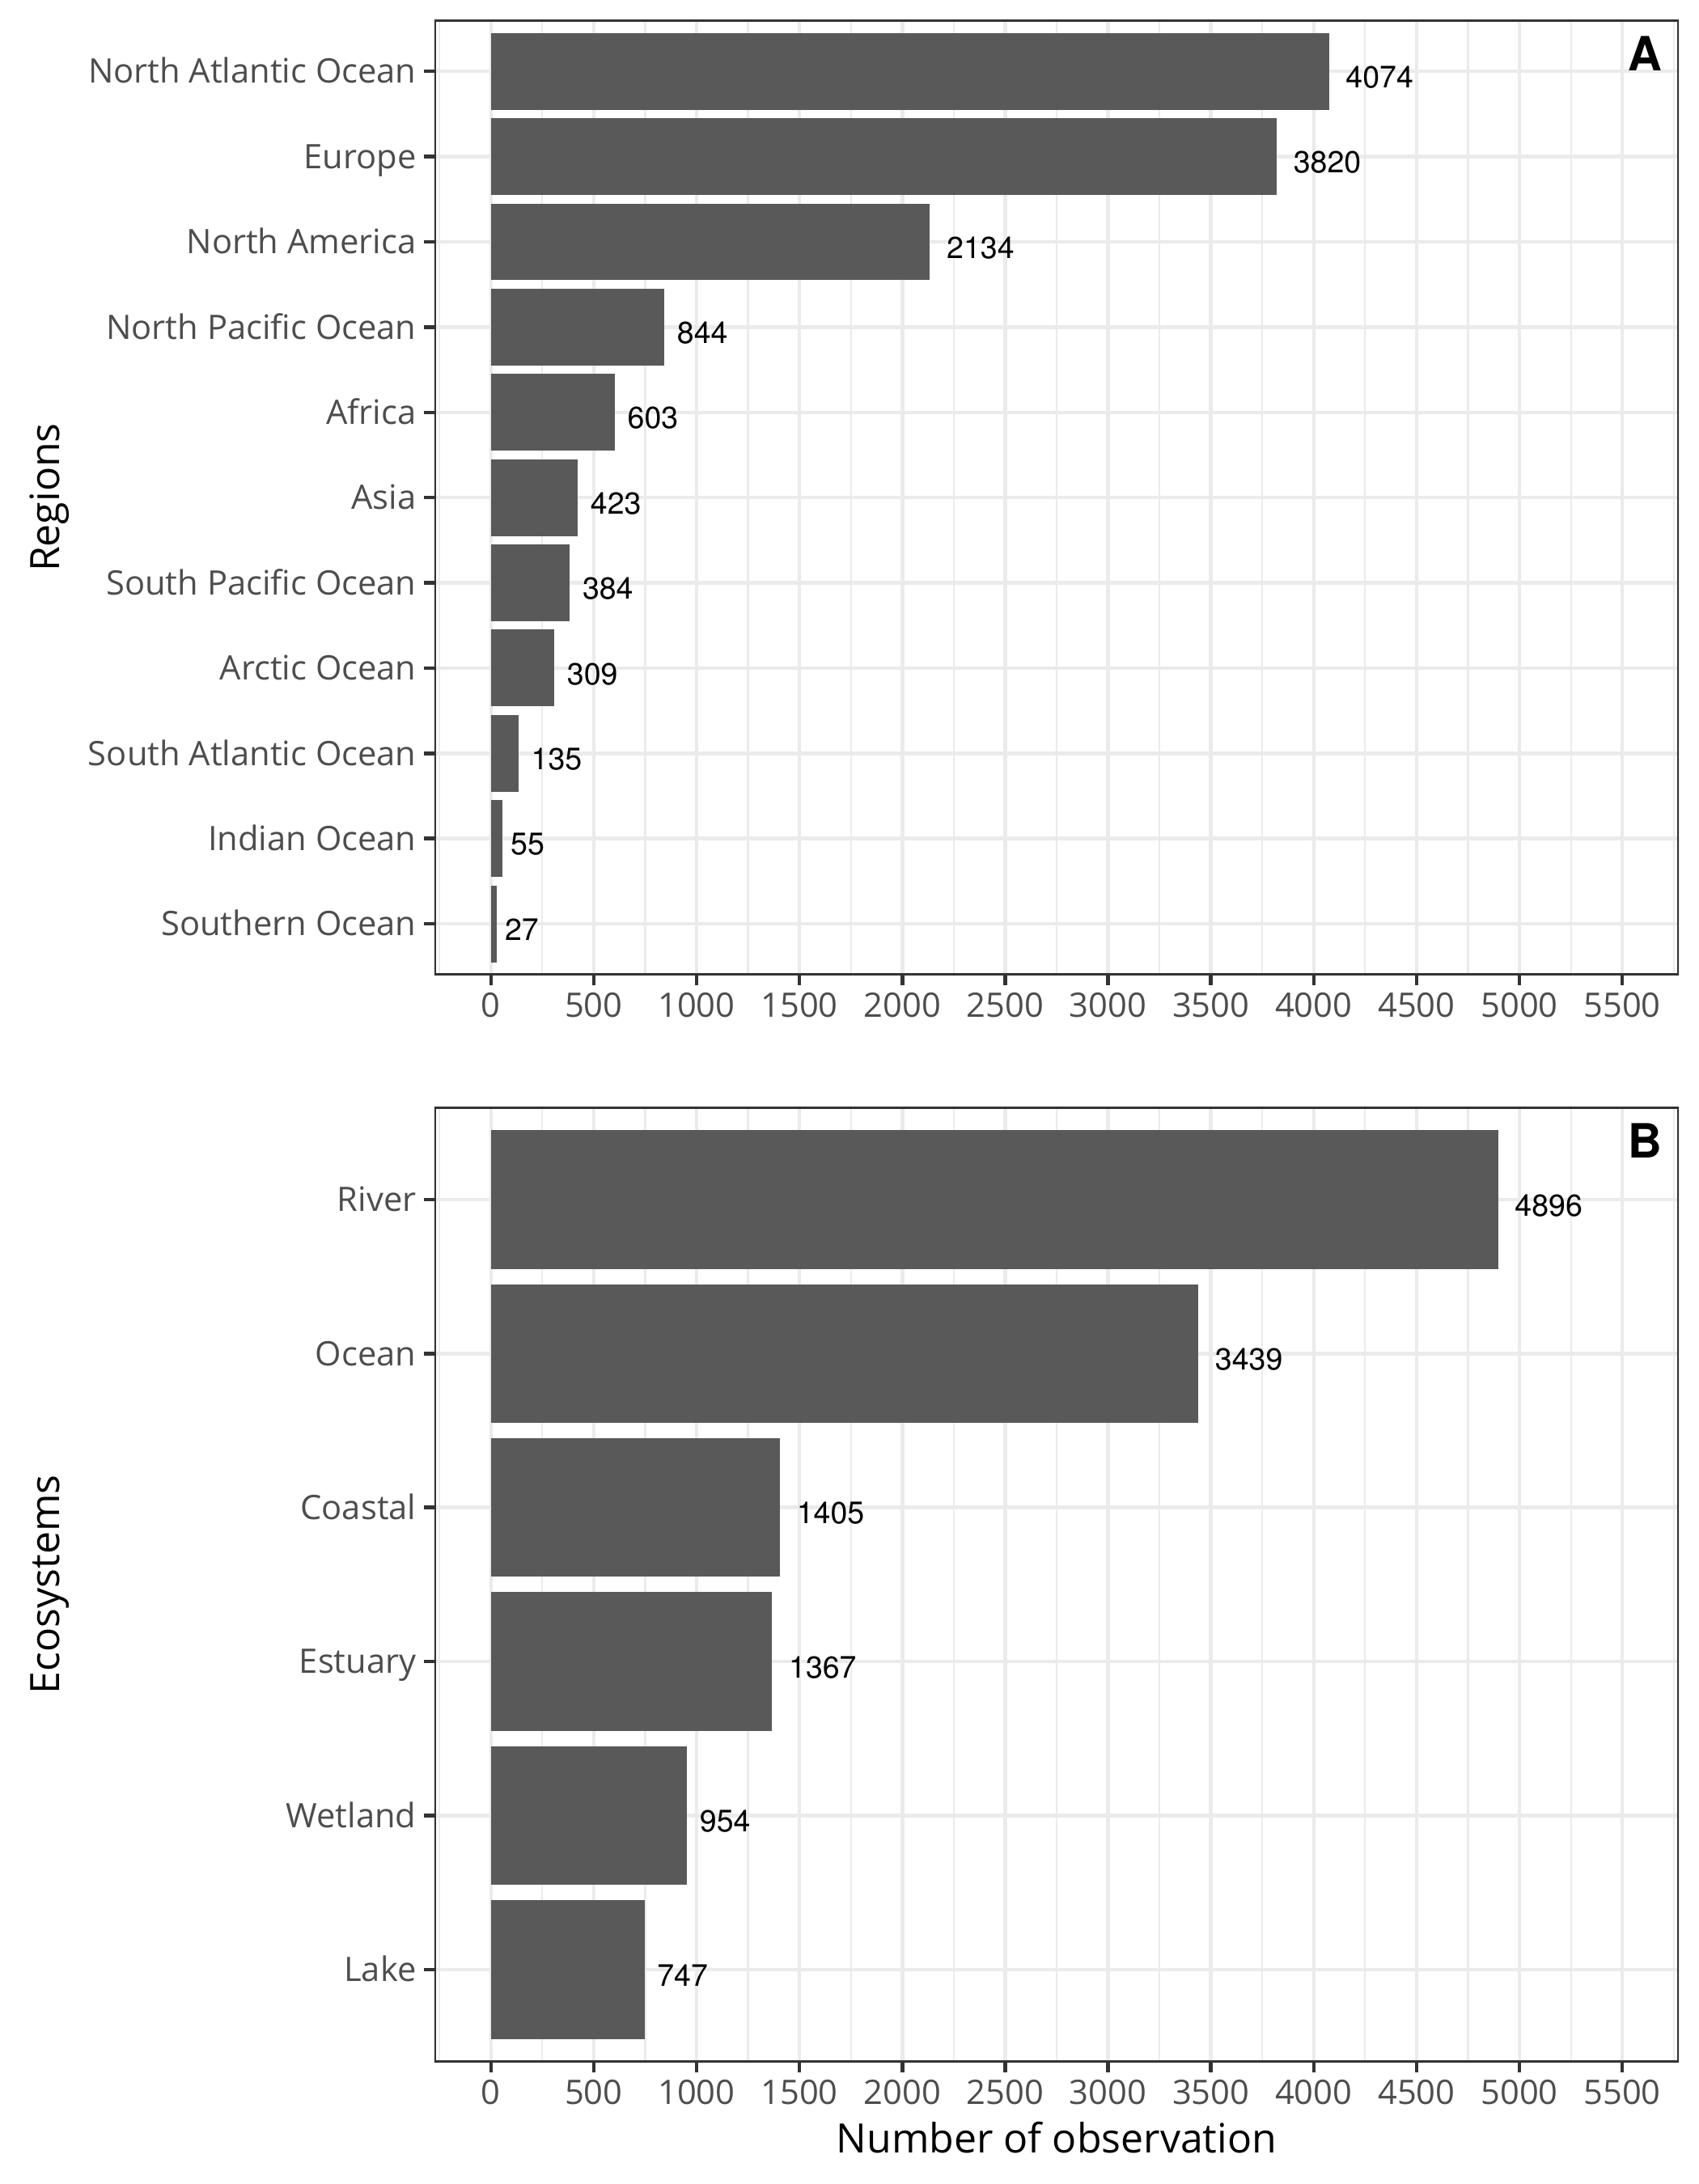
\includegraphics[scale = 1]{../../graphs/appendix1}
	\caption{Barplot showing the number of unique observations in each ecosystem.}
\end{figure}

\clearpage
\newpage

\begin{figure}[h]
	\centering
	\includegraphics[scale = 1]{../../graphs/appendix2}
	\caption{Heat map showing the determination coefficients ($R^2$) of the linear regressions between absorption values for each pair of wavelengths between 250 and 500 nm ($n = 63001$). Each regression is based on 2194 observations. Note that the diagonal of the plot shows $R^2 = 1$.}
\end{figure}

\clearpage
\newpage

\begin{figure}[h]
	\centering
	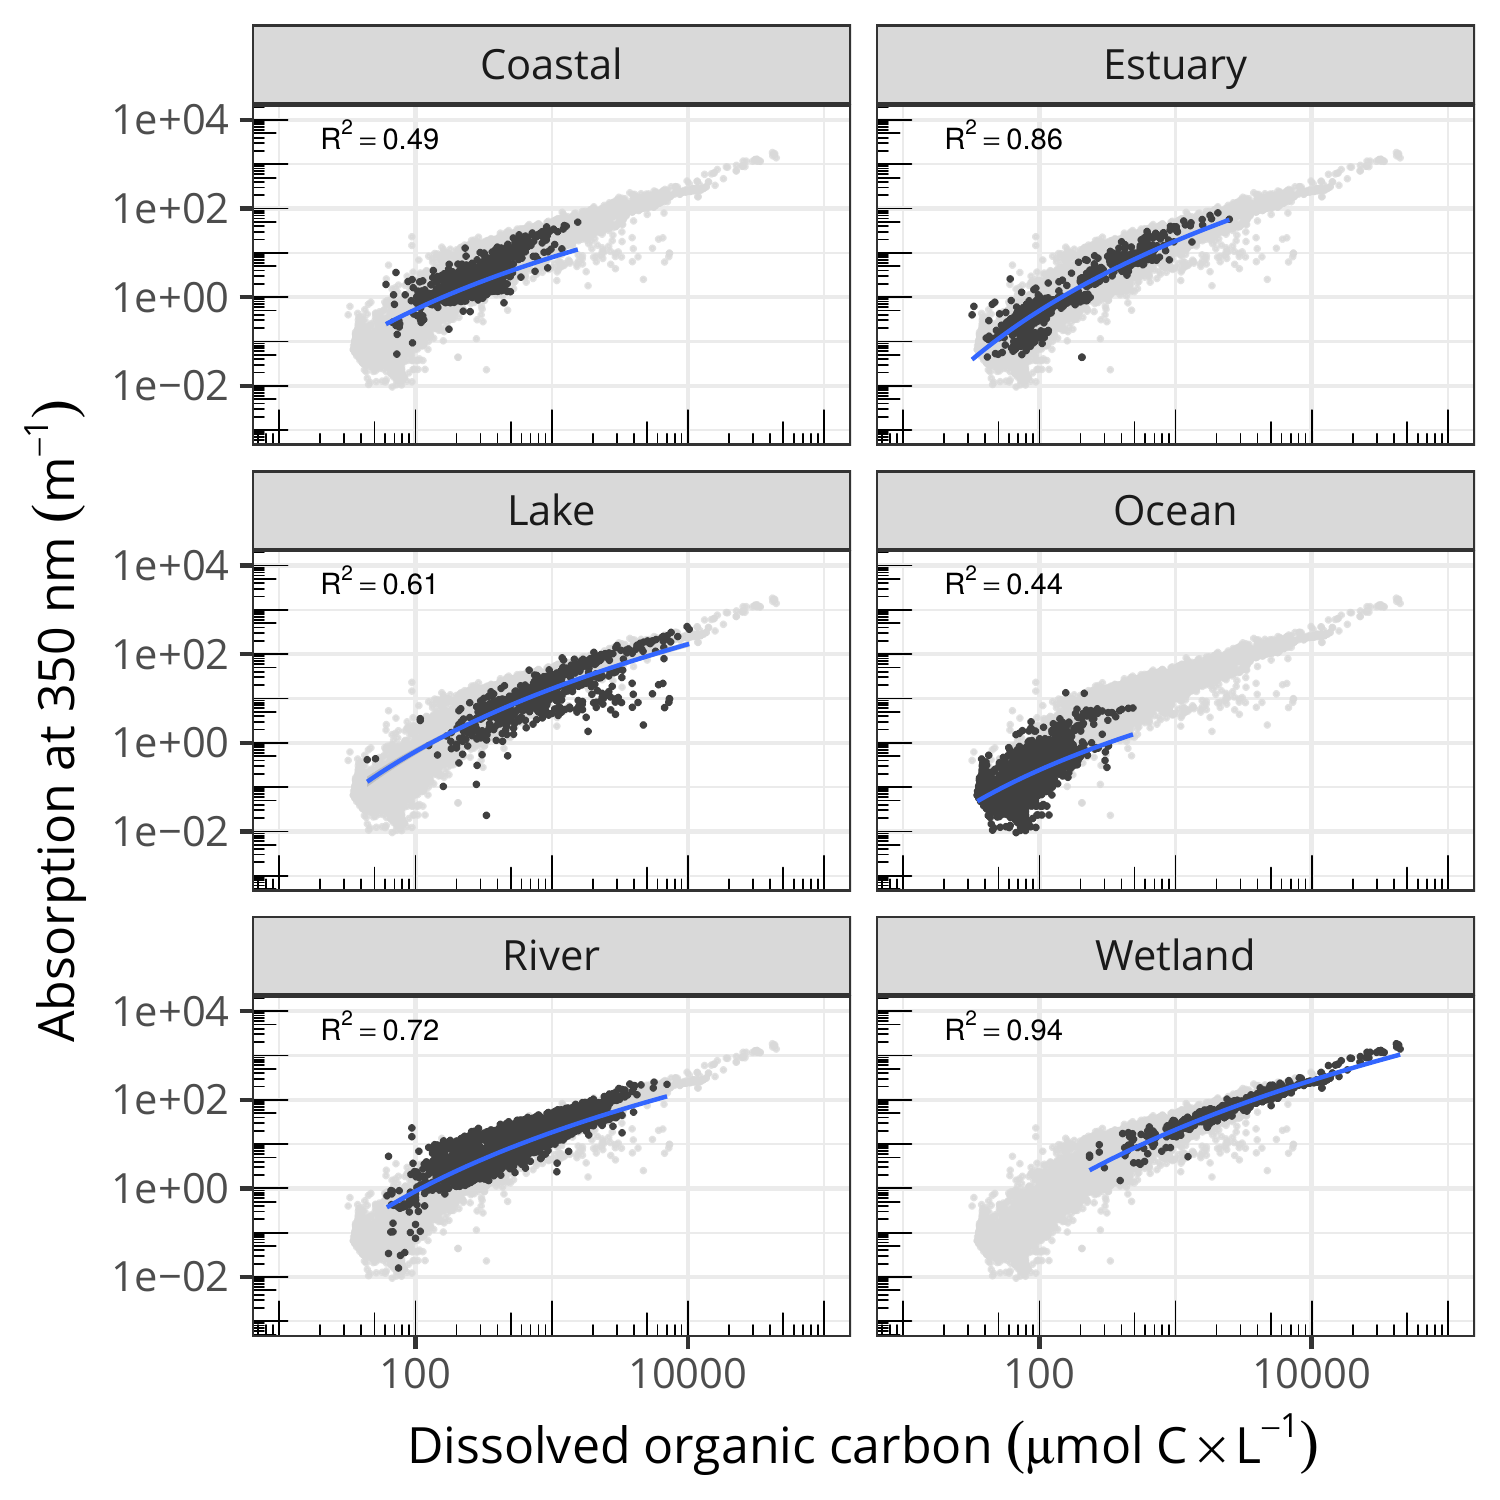
\includegraphics[scale = 1]{../../graphs/appendix3}
	\caption{Log-linear relationship bewteen $a_{CDOM}(350)$ and DOC divided by ecosystems. The blue line is the fitted values of a linear model $y = log(x)$. The shaded areas repesent the 95\% confidence intervals.}
\end{figure}

\clearpage
\newpage

\begin{figure}[h]
	\centering
	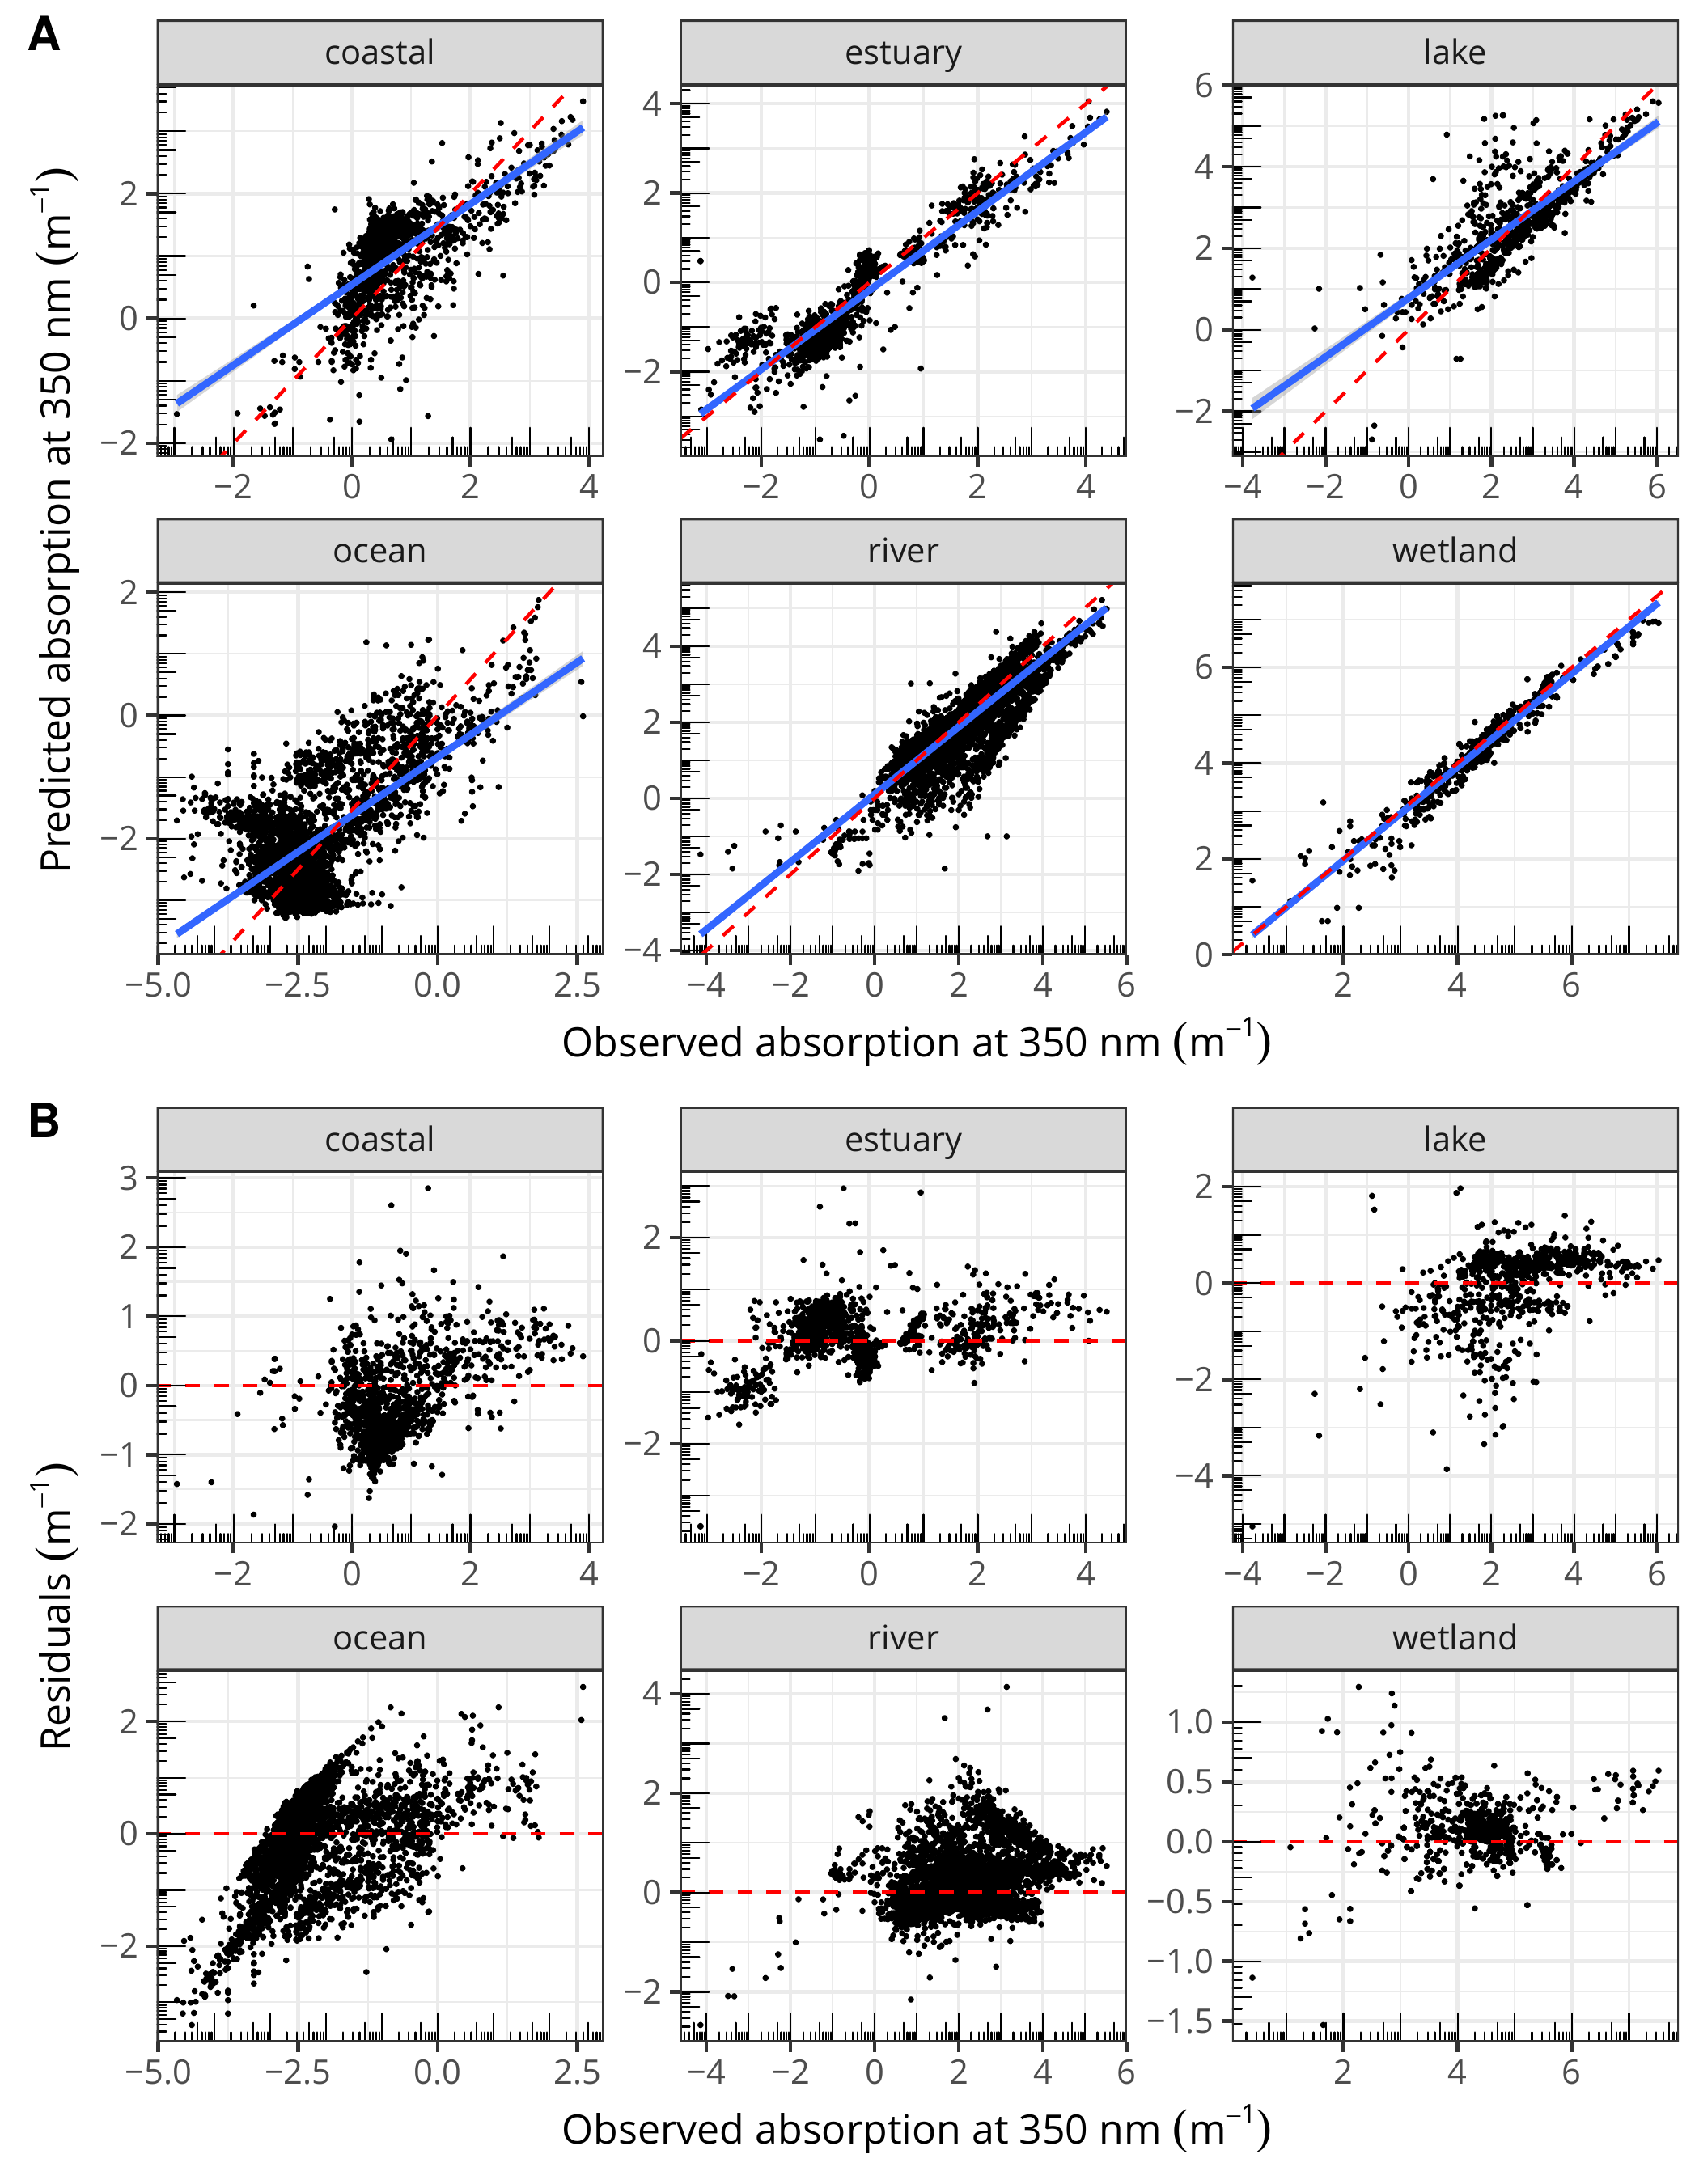
\includegraphics[scale = 1]{../../graphs/appendix4}
	\caption{Power regression between molecular weight and spectral slope calculated between 300 and 600 nm $(S_{300-600})$. Data have been extracted from Stedmon 2015. One outlier was removed from the analysis. Equation of the model: $y = 205.81x^{-0.26}, R^2 = 0.88, n = 62$.}
\end{figure}


\end{document}
